%TODO synthèse
%TODO glossaire et bibliographie etc ..

%%%%%%%%%%%%%%%%%%%%%%%%%%%%%%%%%%%%%%%%%%%%%%%%%%%%%%%%%
%                      Préambule                        %
%%%%%%%%%%%%%%%%%%%%%%%%%%%%%%%%%%%%%%%%%%%%%%%%%%%%%%%%%

%%%%%%%%%%%%%%%%%%%%%%%%%%%%%%%%%%%%%%%%%%%%%%%%%%%%%%%%%%%%%%%%%
%                      Préambule type                          %
%%%%%%%%%%%%%%%%%%%%%%%%%%%%%%%%%%%%%%%%%%%%%%%%%%%%%%%%%%%%%%%%



\def\changemargin#1#2{\list{}{\rightmargin#2\leftmargin#1}\item[]}
\let\endchangemargin=\endlist 

%%%%%%%%%%%%%%%%%% Classe dudit Document %%%%%%%%%%%%%%%%%%%%%%%
\documentclass[a4paper,12pt,openany]{report} % sert à définir des propriétés e base sur les articles
% Autre paramètres connnus: 	*book => pour de vrais livres
%				*article pour des artiles dans des revues scientifiques, des présentations, des rapports courts, des documentations, des invitation etc....
%				*report por des rapports plus long contenant plusieurs chapitres, des petits livres, des thèses
%				*Slides pour des transparants
%				*foiltex
% Option: Xpt taille de la police,  4apaper/letterpaper/a5paper/b5paper/executivepaper, fleqn, leqno, titlepage/notitlepage indique si une nouvelle page doit être commencée après le titre du document, twocolumn,twoside/oneside,



%%%%%%%%%%%%%%%%%%%%%%%% Package %%%%%%%%%%%%%%%%%%%%%%%%%%%%%%%
\usepackage{doc}% permet de documenter des programmes (cf doc.dtx]
\usepackage{exscale} % fournit des version de taille de caractère que LaTeX va utiliser (cf ltexscale.dtx)
\usepackage{fontenc} % spécifie le codage des police de caractère que LaTeX va utiliser (cf ltoutenc.dtx)
%\usepackage[latin]{inputenc} %Autorise les caractères acentués
\usepackage{ifthen} % fournit des commandes de conditions (cf ifthen.dtx)
\usepackage{latexsym} %permet l'utilisation de la police des symboles LaTeX
\usepackage{makeidx} %fournit des commandes pour réaliser un index
\usepackage{syntonly} % analyse le doc sans le formater
\usepackage[T1]{fontenc}
\usepackage[utf8x]{inputenc} 
%\usepackage[utf8]{inputenc}% permet de spécifier le codeage des caractère utiliser dans le source.
\usepackage[english,francais]{babel}
%\usepackage{asmath} %Fonctions servant à l'écriture mathématique
\usepackage{xspace} %Fonctions permettant d'introduire des espaces
\usepackage{xargs} %Permet d'utiliser de définir plus simplement des fonctions
\usepackage{trace}%Permet d'utiliser des traces de debbug
\usepackage{show2e}% debbug
\usepackage[pdftex]{graphicx}
\usepackage{hyperref}

%%%%%%%%%%%%%%%%% Style du pied de page %%%%%%%%%%%%%%%%%%%%%%%%

\pagestyle{plain}% imprime le numéro de page au milieu du pied de page
%\pagestyle{heading}%imprime le titre du chapitre courant et le numéro dans l'en tête et laisse le pied de page vide.
%\pagestyle{empty}% laisse l'en tête et le pied de page vide


%Nota bene: On peut changer le pied de page en court en utilisant \thispagestyle


%%%%%%%%%%%%%%%%% Césure   %%%%%%%%%%%%%%%%%%%%%%%%

\hyphenation{FORTRAN}
\hyphenation{An-ti-cons-ti-tu-tion-nel-le-ment}

%%%%%%%%%%%%%%%% Citation Environement %%%%%%%%%%%%

\newsavebox{\nomepigraphe}
\newenvironment{epigraphe}[1]
	{% clause begin
	\vspace*{-1.5cm}%
	\small\sffamily% mise en évidence
	\savebox{\nomepigraphe}{#1}% une boîte pour sauvegarder
	% l’ origine de la citation
	\slshape% tout est penché
	\begin{changemargin}{0pt}{-2cm}% on se met au large
	\begin{flushright}}% tout est poussé à droite
	{% clause end
	\\[4pt]\usebox{\nomepigraphe}.% insertion de l’origine
	\end{flushright}%
	\end{changemargin}\par\vspace*{0.6cm}}

%
\input ./preambule.tex %sans saut de ligne


%%%%%%%%%%%%%%Titre%%%%%%%%%%%%%%%%%%%%%%%%%%%%%%%%%%%%
\title{ Projet de 3 année à l'INSA Centre Val de Loire } % Titre du document
\author{BAIZ Mamoune && BAIZ Mamoune} % Auteur
\date{\today} % Date de création


%%%%%%%%%%%%%%%%%%%%%%%Debut Doc%%%%%%%%%%%%%%%%%%%%%%%
\begin{document} % Début du document
%%%%%%%%%%%%%%%%%%%%%%Page de Garde%%%%%%%%%%%%%%%%%%%%
{
\begin{titlepage}
  \begin{sffamily}
  \begin{center}

    % Upper part of the page. The '~' is needed because \\
    % only works if a paragraph has started.
    
\includegraphics[scale=0.5]{Images/png/insa_logo.png}~\\[1.5cm]

    \textsc{\LARGE Institut National des Sciences Appliquées  Centre Val de Loire }\\[2cm]

    \textsc{\Large Rapport de projet 3\up{ème} année option 2SU}\\[1.5cm]

    % Title
%    \HRule \\[0.4cm]
    { \huge \bfseries Domotique\\[0.4cm] }

%    \HRule \\[2cm]
    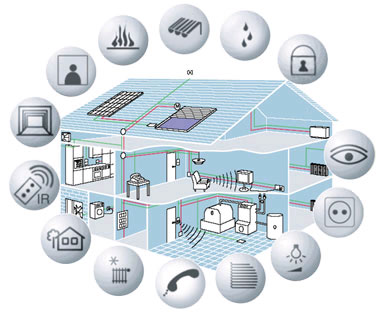
\includegraphics[scale=0.5]{Images/jpg/domotic.jpg}
    \\[2cm]

    % Author and supervisor
    \begin{minipage}{0.4\textwidth}
      \begin{flushleft} \large
        BAIZ Mamoune et MUNIER Marc \\
        Promo 2016\\
      \end{flushleft}
    \end{minipage}
    \begin{minipage}{0.4\textwidth}
      \begin{flushright} \large
        \emph{Encadrant :} M. Briffaut\\
      \end{flushright}
    \end{minipage}

    \vfill

    % Bottom of the page
    {\large 9 Février 2016}

  \end{center}
  \end{sffamily}
\end{titlepage}
}
%%%%%%%%%%%%%%%%%%%%%%%Page Vierge%%%%%%%%%%%%%%%%%%%%
\newpage



%%%%%%%%%%%%%%%%%%%%% Remerciment %%%%%%%%%%%%%%%%%%%%
\newpage
\section*{Remerciement}
Au terme de notre formation à L’INSA Centre Val de Loire,et tout au long de ce projet il est nécessaire de remercier :\newline
Tous mes professeurs, ainsi que tout le corps professoral et administratif de notre établissement, auxquels je tiens à rendre hommage pour leurs efforts prodigieux qu’ils n’ont cessé de fournir afin que nous puissions, mes collèges et moi, avoir une formation solide et rigoureuse ; pour leur encadrement tout au long de cette année, et pour leur disponibilité permanente. Je n’oublierais pas de remercier spécialement M.Briffaut pour son soutien tout au long du projet, ainsi que ces précieux cours de "domotique" sur lesquelles nous avons abouti à réaliser ce projet.\newline
%TODO
\clearpage
%%%%%%%%%%%%%%%%%%%%%Résumé%%%%%%%%%%%%%%%%%%%%%%%%%%%
\section*{Résumé}

%%%%%%%%%%%%%%%%%%%%%table des matières%%%%%%%%%%%%%%%
\newpage
\tableofcontents
\clearpage

%%%%%%%%%%%PLAN
%
%I) Introduction ( comment on a fait ce projet, en quoi il consiste, les enjeux )
%Ce projet se présente comme une très bonne expérience sur le plan théorique et pratique, car il permet de concevoir une première %approche sur le monde des objets connectés et plus spécialement en domotiques. Il constitue aussi une occasion unique pour %mettre en évidence le cumul des connaissances sue nous avons acquis tout au long de notre formation spécialisée en sécurité %ubiquitaire.\newline
%De ce fait, notre binôme a décidé de réaliser un projet concernant la domotique. Toutefois, il est nécessaire de définir ce qu'est la %domotique. La domotique est l'ensemble des techniques de l'électronique, de physique du bâtiment, d'automatisme, de %l'informatique et des télécommunications utilisées dans les bâtiments, plus ou moins « interopérables » et permettant de centraliser %le contrôle des différents systèmes et sous-systèmes de la maison et de l'entreprise (chauffage, volets roulants, porte de garage, %portail d'entrée, prises électriques, etc.). La domotique vise à apporter des solutions techniques pour répondre aux besoins de %confort (gestion d'énergie, optimisation de l'éclairage et du chauffage), de sécurité (alarme) et de communication (commandes à %distance, signaux visuels ou sonores, etc.) que l'on peut retrouver dans les maisons, les hôtels, les lieux publics, etc.

%Mamoune
%II)	Presentation du résultat final.
%		A)	les outils ( raspberry + capteur)
%		B)	le Logiciel (domoticz)
%		C)	l'application
% 
%III)	Comment le mettre en place 
%IV)	présentation appronfondie des composants.
%V)		Nos diffficultés difficulté
%VII)	Conclusion
%
%
%Ne pas oublier le glossaire.
%
% chaque partie est à ecrire dans un fichier indépandant du main
% il suffit de rajouter la ligne suivante pour inclure ces écrits
%\input ./maPartie.tex %sans saut de ligne
%
%%%%%%%%%%%%%%%%%%%


%%%%%%%%%%%%%%%%%%%%%%%%%%%%%%%%%%%%%%%%%%%%%%%%%%%%%%
\section{Introduction}

%%%%%%%%%%%%%%%%%%%%%%%%%%%%%%%%%%%%%%%%%%%%%%%%%%%%%%%
\end{document}
